\chapter{Thrust 2: User Interface and Model Generation}\label{chap:thrust2}

With the flexibility afforded by the \Cyclus ecosystem, it is important to
provide tools that allow users to take advantage of this flexibility while
describing a novel fuel cycle.  Without \emph{a priori} knowledge of the
archetypes that will be used in a simulation, there are three main challenges:
(a) ensuring that the fuel cycle represents a physically valid arrangement of
facilities, (b) providing a graphical user interface for arbitrary sets of
archetype parameters, and (c) allowing for different levels of detail as new
archetypes are introduced to avoid overwhelming the user.

A fundamental requirement of this interface is that it presents the design of
a nuclear fuel cycle as a user task.  Prior \glspl{nfcs} require the
intervention of a developer to introduce novel flows of material between
facilities and users are left only with choices of parameters that may
distribute material over those flows.  In the \Cyclus ecosystem, the ad-hoc
introduction of new archetypes can enable new flow paths through the system
that should be easily realizable as user input.  At the same time, a mechanism
must exist to prevent or discourage a user from forming fuel cycle flow paths
that are not physically realistic.  The existence of the \gls{DRE} mitigates
some of the concern for unrealistic flow paths, while a drag-and-drop
interface can be implemented to enable the flexible design of fuel cycles.

Thrust 2, led by Dr. Erich Schneider at the University of Texas - Austin,
tackled these questions in the development of a user interface for building
simulation models.  Working closely with the Thrust 4 team, the Java platform
was chosen for this capability.  A number of design decisions were made to
facilitate user interaction, and testing of this interface was carried out.
The user input tool was originally referred to as Cycic, but was ultimately
incorporated into the broader user interface that also handled output
visualization, known as Cyclist.  Throughout this chapter, the graphical user
capability for building analysis models will be referred to as Cycic.

\section{Platform Choice}

Some consideration was given to the use of Javascript for this functionality
and its implementation within a standard web browser.  Early prototyping was
promising and suggested that it would be possible to support the core
functionality being considered for this tool.  However, a desire for
integration with the data visualization capability ultimately drove the
decision to switch to the Java programming language, based on considerations
discussed in Chapter \ref{chap:thrust4}.

Java provides native support for many of the user interactions necessary to
develop a tool such as this, including file input/output, a standard array of
user interface widgets, drag-and-drop capability, and dynamic arrangement of
visual elements within the window.

\section{Design and Layout}

The bulk of the activity in this thrust focused on the design of different
user interface elements to provide the necessary flexibility, operability and
robustness.  While the visible layout is important, the most important
contributions of this thrust are particular capabilities that are embedded
into that layout to support the user experience.  Each of the following
sections highlights one of those features.

\subsection{Archetype Discovery}

Since each user is free to collect and deploy plugin modules independently, it
is necessary for the user interface to have a mechanism for discovering which
archetypes are available for any given simulation.  This capability is related
to the Thrust 0 work highlighted in section \ref{sec:model_location}.  While a
user is free to place their archetypes anywhere in their filesystem and refer
to them through the fully formed specification, \Cyclus is also able to
catalog all the available archetypes in a standard location, and report their
full specification.  When Cycic is started, it may not be aware of any
archetypes at all, but can invoke the \Cyclus command-line tool to discover
which archetypes are available.

Cycic is also able to perform this function using remote execution servers as
will be described in Chapter \ref{chap:thrust5}.  In this case it connects to
the remote server and invokes its copy of \Cyclus to query which archetypes
are available on that server.  This allows users to easily switch to different
execution servers, including their local computer or any other publicly
accessible remote server, and determine what kind of archetypes are available.

Once the list of archetypes is discovered, the user interface itself is
updated.  A drop-down list of all available archetypes is populated with the
information that is returned from these queries, forming a catalog of possible
archetypes that a user can choose to include in their model.

\subsection{Drag \& Drop}

To use a particular archetype, the user first selects it from the catalog of
discovered/available archetypes, placing an icon for that archetype in a
``corral'' that is then available for inclusion in the model.  Simply
selecting an archetype is only the first step since the same archetype can be
configured in multiple ways to produce different prototypes, each with the
same underlying behavior but different parameters.  A fuel cycle design is
populated with prototypes. For each prototype, the appropriate archetype is
added by dragging and dropping its icon from the corral into the fuel cycle
design canvas.  Once dropped, these prototypes can be moved around by dragging
and dropping to improve the visual layout of the developing fuel cycle.

To configure a prototype, a double-click will open a window that contains
widgets for the input of each parameter that must be defined for that
archetype, including a name that allows for that prototype to be distinguished
from other prototypes of the same archetype.  Since Cycic has no prior
knowledge of archetype definitions, this must be generated automatically, as
described in the next section.

The default representation of archetypes and prototypes is a colored circle,
in which the color is automatically determined from the archetype
specification.  This leads to unique colors for each archetype that permits
easy identification of the archetypes being used at any time.  It is also
possible to define sets of icons that will be used to represent different
archetypes and prototypes as they are assigned to specific niches in the fuel
cycle.

\subsection{Automated Input Generation}

An important feature related to the automated discovery of archetypes is the
ability to automatically generate graphical user interface capability for each
archetype.  This functionality relies heavily on the metadata discussed in
section \ref{sec:metadata}.  Specific metadata annotations have been defined
for use by the user interface to enable this.  Some of these annotations allow
the archetype developer to specify strings that will be displayed as part of
the user interface as documentation(e.g. \texttt{alias, uilabel, units, doc,
  tooltip}), while others provide semantic information:
\begin{itemize}
\item \textbf{\texttt{type}} describes the C++ implementation of this data
  type and can be used to arrange input widgets in the window for complex data
  types.  For example, if the input quantity is a \texttt{std::map< int key,
    double value>}, the input can be represented as a lists of pairs of input
  boxes, in which each pair represents a single key/value pair, and button to
  add more pairs as necessary.
\item \textbf{\texttt{uitype}} provides a hint about how this variable should
  be displayed for user input.  Some of these indicate that user input for
  this variable should be a drop-down list populated by other elements of the
  model: \texttt{incommodity}, \texttt{outcommodity}, \texttt{facility},
  \texttt{prototype}, \emph{etc}.  \texttt{combobox} specifies a more generic
  drop-down list that will be populated by items specified in the
  \texttt{categorical} metadata, while \texttt{range} specifies that this
  input element should be selected from a continuous variable between the
  values specified in the \texttt{range} metadata.
\item \textbf{\texttt{range}} provides the valid range for an input quantity,
  allowing archetype developers to ensure that only valid quantities are
  given.
\item \textbf{\texttt{categorical}} provides the list of discrete quantities
  that are valid when the \texttt{uitype} is specified as \texttt{combobox},
  allowing archetype developers to constrain the possible choices of a
  variable to those that are consistent with the models implemented in the
  archetype.
\item \textbf{\texttt{default}} provides a default quantity for the input
  data, allowing the input widget for this variable to already be populated
  with that value.  The user can still choose to change the value, but
  immediately sees the default.
\item \textbf{\texttt{internal}} indicates that this variable should not appear
  in the user input or Cycic interface.  This is reserved for quantities that
  are otherwise stored in the database, but are initialized indirectly from
  other user input quantities or default values.
\end{itemize}

Cycic implements code that makes specific design choices based on the values
specified in this metadata.  It is able to query this metadata using the
\Cyclus command-line, whether the archetypes reside on the local computer or
on a remote execution server.

\subsubsection{Expert Level}

One additional metadata annotation is used to provide a specific target
capability: varying levels of complexity for users with varying
sophistication.  The \texttt{userlevel} data is an integer from 0 to 10.  The
user can select their user level, from 0 (simplest) to 10 (most complex), and
will only see input widgets that correspond to variables with that user level
or lower.  All variables with a user level greater than 0 must have a default
value.  This feature allows archetype developers to encode reasonable defaults
for some variables and only allows users to change those values if they have
made a conscious decision to access a higher user level.

At this time, the overall design and layout of Cycic does not change with the
user level, but this would also be possible.  This would allow a completely
different look and feel for different user levels in addition to, and possibly
informed by, the different set of input data that users are asked to provide.

\subsection{Commodity Connections}

Both conceptually and graphically, prototypes are connected in a nuclear fuel
cycle via the commodities that they share.  By definition, a commodity does
not have any particular quality/composition in \Cyclus, but serves to define
the markets in which each agent will participate.  A user gets to decide which
prototypes will serve as consumers and/or suppliers for each commodity in the
problem.  \Cyclus uses the notion of commodity to partition the \gls{DRE} into
smaller network flow problems that can be solved independently and more
efficiently.  These commodities also result in visual information in the form
of arrows that connect prototypes in the fuel cycle design canvas.

In an effort to ensure that the user designs a viable fuel cycle, this
information also provides hints to the users about the allowable flows of
material among the prototypes that they are placing into the model.  It is
important to recognize that these are only hints as it doesn't prevent the
user from designing a fuel cycle that violates physics.  It is, however, up to
the agency defined in each facility's archetype to manage its interactions
with the \gls{DRE}, and prevent unphysical results from arising.

\subsection{Sample}

Figure \ref{fig:cycic-sample} shows a partially defined fuel cycle that
includes a mine, an enrichment facility and a reactor, using a set of icons
based on \gls{USDOE} graphics for fuel cycles\citeref{dixon_dynamic_2008}.  In
this case, the available archetypes have been discovered on the remote \Cyclus
execution server at the address \texttt{http://cycrun.fuelcycle.org}. The
uranium mine, enrichment facility and reactor are based on the
\texttt{Source}, \texttt{Enrichment}, \texttt{Reactor} archetypes,
respectively, provided by the \Cycamore library.  At the right is the
auto-generated user input panel, at user level 0, for the reactor prototype
with the name ``ALWR''.  The commodity ``U-ore'' is produced by the mine and
consumed by the enrichment facility while ``Fresh-UOX-Fuel'' is produced by
the enrichment facility and consumed by the reactor.  Note that this latter
commodity does not have a specific composition, but that the reactor facility
defines a specific recipe, ``Fresh-UOX-Fuel-4'' that it will request to
satisfy this commodity need.

\begin{figure}[htbp]
  \centering
  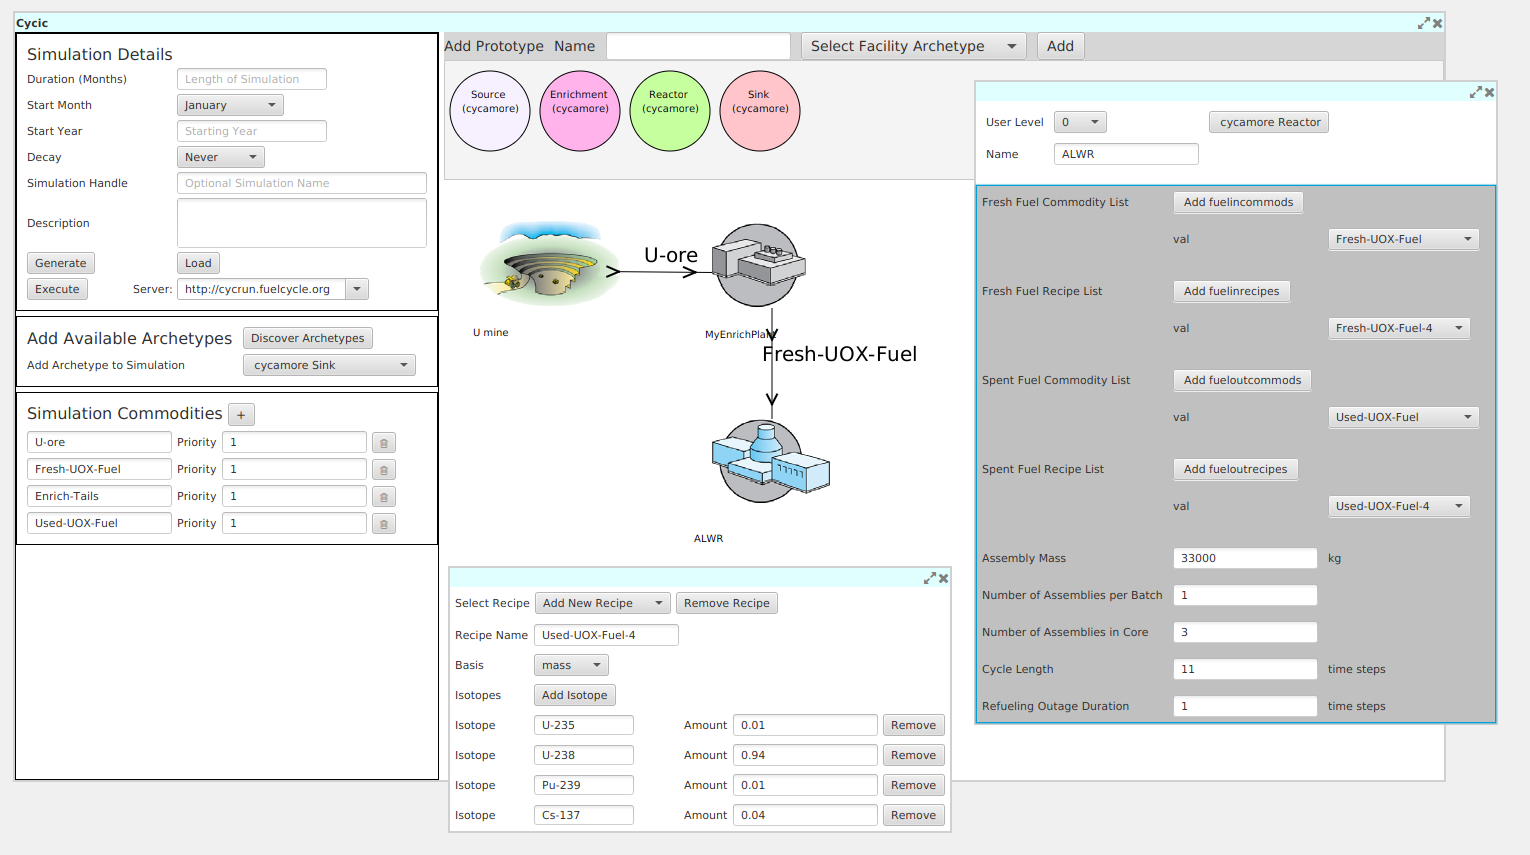
\includegraphics[width=\columnwidth]{./images/cycic-sample}
  \caption{A screenshot of the Cycic user interface in the middle of defining a simple fuel cycle.}
  \label{fig:cycic-sample}
\end{figure}

\section{User Experience Testing}

The Thrust 2 team embarked on user experience testing to determine how well
the implemented design of Cycic met the needs of users working to design
nuclear fuel cycles.

The first round of testing relied on a group of graduate students in nuclear
engineering.  The users were given a tutorial consisting of a brief
introduction to the concepts of \Cyclus while demonstrating how they were
represented in the Cycic user interface.  Most users viewed this tutorial once
as a group and again individually immediately prior to testing their user
experience.

Users were given a task to complete using the software and their actions were
tracked by an observer while they also narrated their actions and decisions.
The technique of self-narration allows users to comment on things that might
not arise in questioning, and also allows the user to complete the task
without the interruption of questions.  The primary data recorded by the
observer was the amount of time and number of mouse clicks required by the
user in each step of the task.

Each participant was to construct a simple fuel cycle consisting of three
prototypes - a source, a reactor and a sink - and add other components
necessary for a full \Cyclus simulation: an institution and a region.
Following the task each participant was asked four questions and invited to
make additional comments.  These four questions focused on specific contrasts
that were introduced during the task phase:
\begin{itemize}
\item text-based prototype creation vs drag-and-drop
\item corral view of regions vs text form of institutions
\item the benefit of choosing a low user level
\item the clarity of presenting defaults for advanced user level data
\end{itemize}

The two principal findings of the observations and self-narration were that
(a) users were confused about the difference/relationship between institutions
and regions, and (b) the text-based institution view was more challenging to
understand than the corral-based view of the region interface.  While the
first of these is a core \Cyclus concept and not specific to the user
interface, the user interface could be modified to explicitly support a better
understanding of the \gls{RIF} hierarchty.  The second finding suggests that
the manipulation of institutions should be modified to be more like the region
corral view. Two additional, more minor findings were that new prototypes
should have a default name, rather than no name at all, and that a better mode
for connecting facilities via commodities would be valuable.

Regarding the specific follow up questions, the majority of users (10/13)
preferred the drag-and-drop method for adding prototypes, and some of those
who indicated a preference for text entry acknowledged that drag-and-drop may
be preferred for learning a new tool.  Nearly all of the users (12/13)
preferred the corral view for regions over the text form for institutions.
All users found the presence of user levels made the tool easier to use,
reducing clutter and preventing information overload.  All users felt that it
was clear that values that populated the input widgets when the user level was
increased constituted default values.

The software was updated prior to a second round of testing.  Specifically,
the institution view was updated to behave similarly to the region view, both
now relying on an updated corral view with drag and drop capability from
available archetypes.  In addition, the region view now also includes a list
of unassociated institutions to reinforce the relationship between regions and
institutions.  Tooltips (small documentation that appears when the mouse
hovers over an input widget) were added to the region and institution views,
and popup help windows were implemented with longer documentation for most
windows and widgets.

A similar tutorial was given prior to the user experience testing in this
second round.  The task again required users to build a fuel cycle model, but
this time with more complexity.  The facility prototypes consisted of three
sources, a fuel fabrication plant, a reprocessing plant, two different
reactors, and sink.  The institution was configured to build reactors of each
kind at three different points in time.  This more complex scenario was
constructed to provide more time for observation and self-narration.  In
addition observing the time spent and number of clicks in each view, the
observer also recorded the number of times that the user switched between two
open views.

Fifteen users were again asked a series of questions following the exercise.
For those users who had participated in the previous test, they were asked to
rate the changes.  Those users new to Cycic were asked to rate the same
features as in the first test, as well as the new features represented by the
software changes.  All participants were asked how each view helped to
understand \Cyclus itself and to rate different widget choices.  Finally,
participants were solicited for any improvements that they wold recommend.

The average time to complete the task was about 20 minutes (range: 16-30
minutes), nearly 2 times longer than an expert user as represented by the
software developer.  The majority of this time (12 min) was spent in the
configuring the facilities in their respective form views, but the range of
times was narrowest, with the slowest user only taking 72\% longer than the
fastest.  The recipe view provided the most challenge, in this respect, with
the slowest user spending nearly 6 times longer than the fastest person.

The most significant difference between the expert time to complete and the
users was with the institution form.  While the ratio of 3.7 was similar to
that in the region view (3.8), the time spent in the institution view
represented a substantial larger fraction of the total (3.5 min vs 1 min).
Through questioning, the users indicated that the specific purpose of this
institution archetype was unclear and thus the requested data was also
unclear.

Combining the observed interactions with the responses to the post-exercise
questions, much of the feedback of the second round of testing was consistent
with the first round.  Returning users recognized the improvements in the
institution view but still considered one of the least clear parts of the
problem definition.  The addition of tooltips was not well received since the
value of information was deemed too low considering the time delay for the
tooltip to appear.

\section{Summary}

A number of design choices were implemented in the Cycic model building
interface to satisfy the need for supporting a flexible plugin ecosystem.
These tools have been demonstrated to support the construction of complex fuel
cycle models.  Testing of the user experience resulted in software
improvements that have been favorably received.
